\documentclass[varwidth]{standalone}
\usepackage{mwe}
\usepackage[labelfont=normalsize,labelformat=parens,
justification=centering]{caption,subfig} %%% Center the caption
\usepackage{amsfonts,amsmath,amssymb}
\usepackage[slovene]{babel}
\usepackage[utf8]{inputenc}
\usepackage[T1]{fontenc}
  
\usepackage{tikz, verbatim}
\usepackage{pgfplots}
\usetikzlibrary{arrows.meta, calc, positioning, automata}

\newcommand{\subdiv}[3] {
\draw ($ 0.5*#2 + 0.5*#3 $) -- #1;
\draw ($ 0.5*#1 + 0.5*#3 $) -- #2;
\draw ($ 0.5*#1 + 0.5*#2 $) -- #3;
}
\begin{document}
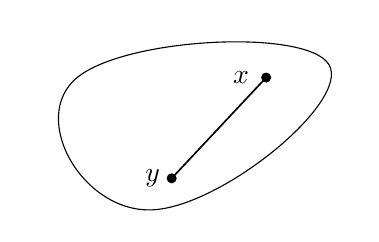
\begin{tikzpicture}[scale=0.8]
		\draw plot [smooth cycle, tension = 1] coordinates {(-2.5, 0.3) (-1.3, -1.8) (1.5, 0.5)};
		\filldraw (0.5, 0.3) circle (2pt);
		\filldraw (-1, -1.3) circle (2pt);
		\draw[line width=0.6pt] (0.5, 0.3) -- (-1, -1.3);
		\draw (0.1, 0.3) node {$x$};
		\draw (-1.3, -1.3) node {$y$};
		\end{tikzpicture}%
\end{document}